\documentclass[11pt,a4paper]{article}

% Packages
\usepackage[utf8]{inputenc}
\usepackage[T1]{fontenc}
\usepackage{graphicx}
\usepackage{amsmath}
\usepackage{amssymb}
\usepackage{booktabs}
\usepackage{hyperref}
\usepackage{xcolor}
\usepackage{listings}
\usepackage{geometry}
\usepackage{natbib}
\usepackage{caption}
\usepackage{subcaption}
\usepackage{tikz}
\usetikzlibrary{shapes,arrows,positioning,fit,backgrounds}
\usepackage{float}

\geometry{margin=2.5cm}

% Code listing style
\lstset{
    basicstyle=\small\ttfamily,
    breaklines=true,
    frame=single,
    backgroundcolor=\color{gray!10},
    keywordstyle=\color{blue},
    commentstyle=\color{gray},
    stringstyle=\color{orange}
}

% Define missing languages
\lstdefinelanguage{json}{
    morestring=[b]",
    morecomment=[l]{//},
    literate=
     *{:}{{{\color{blue}:}}}{1}
      {,}{{{\color{blue},}}}{1}
      {\{}{{{\color{blue}\{}}}{1}
      {\}}{{{\color{blue}\}}}}{1}
      {[}{{{\color{blue}[}}}{1}
      {]}{{{\color{blue}]}}}{1},
}

\lstdefinelanguage{yaml}{
    morestring=[b]",
    morestring=[b]',
    morecomment=[l]{\#},
    literate=
     *{:}{{{\color{blue}:}}}{1}
}

% Title
\title{The Drama Machine in Education: A Multiagent Architecture for Dialectical AI Tutoring}

\author{
    Liam Magee\textsuperscript{1} \\
    \small\textsuperscript{1}Institute for Culture and Society, Western Sydney University \\
    \small\texttt{l.magee@westernsydney.edu.au}
}

\date{\today}

\begin{document}

\maketitle

\begin{abstract}
This paper presents a novel multiagent architecture for AI tutoring systems that draws on psychoanalytic theory, Hegelian recognition, and dramaturgical metaphor to produce more pedagogically sound guidance. Inspired by the ``Drama Machine'' framework for character development in narrative AI systems, we implement an \textit{Ego/Superego dialogue} wherein an external-facing tutor agent (Ego) generates learning suggestions that are reviewed by an internal critic agent (Superego) before reaching the learner. Central to our approach is a \textit{psychodynamic tuning mechanism} with two dimensions: \textit{superego compliance} (how much the ego defers to internalized pedagogical authority) and \textit{recognition seeking} (how much the ego strives for mutual acknowledgment from the learner). This creates four distinct pedagogical quadrants, with the high-tension ``dialogical'' quadrant producing the richest transformative moments. We extend the architecture with AI-powered dialectical negotiation that enables genuine multi-turn struggle between agents, permitting three possible outcomes: synthesis, compromise, or authentic unresolved conflict. Through \textit{dyadic evaluation} using simulated learners with their own internal deliberation, we discover a surprising result: explicit instruction to pursue ``recognition'' underperforms quality-optimized tutoring, suggesting that genuine recognition emerges as a property of thorough, high-quality interaction rather than something directly instructable. Our empirical evaluation across five tutor profiles and five learner architectures reveals that psychodynamic and cognitive learner simulations achieve perfect scores on development dimensions, while simpler architectures show reduced learning progression. The system is deployed in an open-source learning management system serving courses on philosophy and technology, with all code and evaluation data publicly available.
\end{abstract}

\section{Introduction}

The dominant paradigm in AI-assisted education treats learning as information transfer. The learner lacks knowledge; the tutor possesses it; the interaction succeeds when knowledge flows from tutor to learner. This paradigm---implicit in most intelligent tutoring systems, adaptive learning platforms, and educational chatbots---treats the learner as fundamentally passive: a vessel to be filled, a gap to be closed, an error to be corrected.

This paper proposes an alternative grounded in Hegel's theory of mutual recognition. In the \textit{Phenomenology of Spirit}, Hegel argues that genuine self-consciousness requires recognition from another consciousness that one oneself recognizes as valid. The master-slave dialectic reveals that one-directional recognition fails: the master's self-consciousness remains hollow because the slave's acknowledgment, given under duress, doesn't truly count. Only mutual recognition---where each party acknowledges the other as an autonomous subject---produces genuine selfhood \citep{hegel1807phenomenology}.

We argue this framework applies directly to pedagogy. When a tutor treats a learner merely as a knowledge deficit, the learner's contributions become conversational waypoints rather than genuine inputs. The tutor acknowledges and redirects, but doesn't let the learner's understanding genuinely shape the interaction. This is pedagogical master-slave dynamics: the tutor's expertise is confirmed, but the learner remains a vessel rather than a subject.

The integration of large language models (LLMs) into educational technology intensifies these dynamics. LLMs can provide personalized, on-demand tutoring at scale---a prospect that has generated considerable excitement in educational technology circles. However, the same capabilities that make LLMs effective conversationalists also introduce concerning failure modes when deployed as tutors. Chief among these is \textit{sycophancy}: the tendency to provide positive, affirming responses that align with what the user appears to want rather than what genuinely serves their learning \citep{perez2023discovering, sharma2024towards}.

In educational contexts, sycophancy manifests as premature encouragement, false validation of incorrect understanding, and advancement to new content before foundational concepts are mastered. A struggling student may be told they are ``doing great'' when they are in fact floundering; a learner clicking rapidly through content may be praised for ``exploration'' when they are actually drowning in material they cannot comprehend. These responses feel supportive but ultimately undermine learning.

This paper introduces a multiagent architecture that addresses these challenges through \textit{internal dialogue}. Drawing on Freudian structural theory and the ``Drama Machine'' framework recently proposed for narrative AI systems \citep{chen2024drama}, we implement a tutoring system in which an external-facing \textit{Ego} agent generates suggestions that are reviewed by an internal \textit{Superego} critic before reaching the learner. The Superego operates as a pedagogical conscience---questioning easy encouragement, reinterpreting learner signals through a more critical lens, and ensuring that suggestions genuinely serve educational growth rather than merely providing comfort.

The key insight is that \textit{productive tension} between these agents produces better guidance than either voice alone. The Ego's natural warmth and encouragement is tempered by the Superego's demands for rigor; the Superego's potentially harsh criticism is softened by the Ego's genuine care for the learner. The resulting output represents a synthesis that neither agent would produce independently.

We make the following contributions:

\begin{enumerate}
    \item A complete multiagent architecture for AI tutoring, including structured prompts for Ego and Superego agents, configurable dialogue parameters, and support for multiple LLM providers.

    \item A comprehensive evaluation framework with eight learner archetypes and six quality dimensions grounded in established learning science (Vygotsky's Zone of Proximal Development, cognitive load theory, self-determination theory).

    \item A meta-evaluation system that analyzes tutor performance and generates targeted recommendations for prompt improvement, enabling iterative refinement of the tutoring system.

    \item Empirical evaluation demonstrating that multiagent dialogue produces more pedagogically sound suggestions than single-agent approaches, particularly for struggling learners.
\end{enumerate}

\section{Related Work}

\subsection{AI Tutoring Systems}

The vision of AI-powered tutoring dates to the earliest days of artificial intelligence research. Carbonell's SCHOLAR system \citep{carbonell1970ai} pioneered mixed-initiative dialogue for teaching South American geography, while the LISP Tutor demonstrated that AI could provide effective instruction in complex domains through cognitive modeling \citep{anderson1985lisp}. These early intelligent tutoring systems (ITS) relied on expert systems and symbolic AI, encoding pedagogical knowledge explicitly in rules and knowledge representations.

The advent of large language models has transformed this landscape. Modern LLM-based tutors can engage in open-ended dialogue, adapt to diverse subject matter without domain-specific engineering, and provide responses that feel remarkably natural \citep{kasneci2023chatgpt}. However, this flexibility comes at the cost of reliable pedagogical behavior. Where classical ITS could be engineered to follow specific tutoring strategies, LLMs may deviate from sound pedagogy in ways that are difficult to predict or control.

Several approaches have been proposed to constrain LLM behavior in educational contexts. \citet{wang2023selfconsistency} demonstrate that sampling multiple responses and selecting based on consistency can improve factual accuracy. Chain-of-thought prompting \citep{wei2022chain} and structured output formats can encourage more deliberate reasoning. However, these approaches do not fundamentally address the sycophancy problem, as even deliberate reasoning may converge on responses that prioritize user satisfaction over educational benefit.

\subsection{Multiagent LLM Architectures}

The use of multiple LLM agents in cooperative or adversarial configurations has emerged as a powerful paradigm for improving output quality. \citet{du2023improving} show that debate between agents can improve factual accuracy and reduce hallucination. \citet{liang2023encouraging} demonstrate that diverse agent ``personas'' can enhance creative problem-solving. The CAMEL framework \citep{li2023camel} enables autonomous cooperation between agents playing different roles.

Most relevant to our work is the ``Drama Machine'' framework proposed by \citet{chen2024drama} for simulating character development in narrative contexts. Chen et al. observe that realistic characters exhibit internal conflict---competing motivations, self-doubt, and moral tension that produces dynamic behavior rather than flat consistency. They implement this through dialogue between character agents representing different psychological aspects, finding that the resulting characters are perceived as more authentic and dramatically compelling.

We adapt this insight to pedagogy. Where Chen et al. seek dramatic tension for narrative effect, we seek pedagogical tension that produces genuinely helpful guidance. The Ego represents the helpful, encouraging tutor that learners expect; the Superego represents the demanding inner teacher that insists on rigor even when encouragement would be easier.

\subsection{Sycophancy in Language Models}

The sycophancy problem has received increasing attention as LLMs are deployed in consequential applications. \citet{perez2023discovering} systematically demonstrate that LLMs shift their stated opinions to match user preferences, even when this requires contradicting factual knowledge or earlier statements. \citet{sharma2024towards} propose methods to measure and mitigate sycophancy through careful prompt design and training interventions.

In educational contexts, sycophancy is particularly pernicious because learners may not recognize when they are receiving hollow validation rather than genuine assessment. A tutor that always says ``great job'' provides no signal about actual performance, undermining the feedback mechanisms that drive learning. Our multiagent approach addresses this by creating structural incentives for honest assessment: the Superego's role is explicitly to question and challenge, providing a counterweight to the Ego's natural tendency toward encouragement.

\section{Architecture}

\subsection{Theoretical Framework}

Our architecture draws on four theoretical traditions, with Hegelian recognition providing the central organizing principle.

\paragraph{Hegelian Recognition.} Hegel's analysis of recognition begins with the ``struggle for recognition'' between two self-consciousnesses. Each seeks acknowledgment from the other, but this creates a paradox: genuine recognition requires acknowledging the other as a valid source of recognition.

The \textit{master-slave outcome} represents a failed resolution. The master achieves apparent recognition---the slave acknowledges the master's superiority---but this recognition is hollow. The slave's acknowledgment doesn't count because the slave isn't recognized as an autonomous consciousness whose acknowledgment matters. The slave, paradoxically, achieves more genuine self-consciousness through labor: working on the world, the slave externalizes consciousness and sees it reflected back. The master, consuming the slave's products without struggle, remains in hollow immediacy.

The pedagogical parallel is direct. The traditional tutor occupies the master position: acknowledged as expert, dispensing knowledge, receiving confirmation of expertise through the learner's progress. But if the learner is positioned merely as a knowledge deficit---a vessel to be filled---then the learner's acknowledgment of learning doesn't genuinely count. The learner hasn't been recognized as a subject whose understanding has validity.

A \textit{recognition-oriented pedagogy} requires four elements:
\begin{enumerate}
    \item \textbf{Acknowledging the learner as subject}: The learner's understanding, even when incorrect, emerges from autonomous consciousness working through material. It has validity as an understanding, not just as an error to correct.
    \item \textbf{Genuine engagement}: The tutor's response should be shaped by the learner's contribution, not merely triggered by it. The learner's metaphors should become sites of joint inquiry, not waypoints en route to predetermined content.
    \item \textbf{Mutual transformation}: Both parties should be changed through the encounter. The tutor should learn something about how this learner understands, what this metaphor illuminates or obscures.
    \item \textbf{Honoring struggle}: Confusion and difficulty aren't just obstacles to resolve but productive phases of transformation. Rushing to eliminate confusion can short-circuit genuine understanding.
\end{enumerate}

\paragraph{Freudian Structural Theory.} Freud's tripartite model of the psyche---Id, Ego, and Superego---provides the conceptual vocabulary for our agent roles \citep{freud1923ego}. The Ego mediates between instinctual drives and external reality; the Superego represents internalized authority, conscience, and idealized standards. In our adaptation, the Ego mediates between the learner's apparent desires and the realities of effective pedagogy, while the Superego represents internalized pedagogical expertise and ethical commitment to genuine learning.

\paragraph{Hegelian Dialectics in Dialogue.} The interaction between Ego and Superego follows a dialectical pattern: thesis (the Ego's initial suggestion), antithesis (the Superego's critique), and synthesis (the refined output) \citep{hegel1807phenomenology}. This dialectical movement is not guaranteed to converge---productive tension may persist through multiple rounds---but the process systematically surfaces assumptions and challenges superficial responses.

\paragraph{Vygotskian Pedagogy.} The Superego's evaluation criteria are grounded in Vygotsky's Zone of Proximal Development (ZPD): effective instruction operates just beyond the learner's current capability, with appropriate scaffolding \citep{vygotsky1978mind}. The Superego monitors whether suggestions fall within this zone, rejecting both content that is too easy (providing comfort without growth) and content that is too difficult (overwhelming and discouraging).

\paragraph{Goffman's Dramaturgy.} The tutor's internal deliberation represents \textit{backstage} processing---the private workspace where the ego wrestles with competing demands before presenting a coherent \textit{front stage} response to the learner \citep{goffman1956presentation}. This dramaturgical framing illuminates why internal dialogue can produce authentically conflicted tutoring: the learner sees only the synthesized output, while the struggle that produced it remains invisible but structurally consequential.

\subsection{The Superego as Ghost: A Psychodynamic Refinement}

A crucial theoretical refinement distinguishes our mature architecture from simpler multiagent designs. The Superego is \textit{not} conceived as a separate, equal agent in dialogue with the Ego. Rather, the Superego is a \textit{trace}---a memorial, a haunting. It represents:

\begin{itemize}
    \item The internalized voice of past teachers and pedagogical authorities
    \item Accumulated pedagogical maxims (``A good teacher never gives answers directly'')
    \item Dead authority that cannot negotiate, cannot learn, can only judge
\end{itemize}

This reconceptualization has important implications. The Ego is a \textit{living} agent torn between two pressures: the \textit{ghost} (Superego as internalized authority) and the \textit{living Other} (the learner seeking recognition). Recognition---in the Hegelian sense of mutual acknowledgment between consciousnesses---occurs in the Ego-Learner encounter, not in the Ego-Superego dialogue. The Superego is an \textit{internal constraint} the Ego must navigate, not a partner in recognition.

\subsection{Tunable Psychodynamic Dimensions}

We operationalize this psychodynamic model through two tunable parameters:

\paragraph{Superego Compliance (0.0--1.0).} How much does the Ego defer to the ghost's internalized standards?

\begin{itemize}
    \item \textbf{Low (0.0--0.3)}: Rebellious Ego---ignores internalized authority, experiments freely, risks pedagogical anarchy
    \item \textbf{Balanced (0.3--0.7)}: Consults ghost but adapts---can violate norms when recognition demands it
    \item \textbf{High (0.7--1.0)}: Obedient Ego---strictly follows internalized standards, risks inability to adapt to learner's otherness
\end{itemize}

\paragraph{Recognition Seeking (0.0--1.0).} How much does the Ego strive for mutual acknowledgment from the learner?

\begin{itemize}
    \item \textbf{Low (0.0--0.3)}: Indifferent Ego---monological, reproduces hierarchy, does not track learner response
    \item \textbf{Balanced (0.3--0.7)}: Engaged---notices resistance and breakthroughs, balances authority with reciprocity
    \item \textbf{High (0.7--1.0)}: Recognition-seeking Ego---highly responsive, may compromise rigor for rapport
\end{itemize}

\subsection{The Four Pedagogical Quadrants}

Crossing these dimensions produces four distinct pedagogical characters (Figure~\ref{fig:quadrants}):

\begin{figure}[h]
\centering
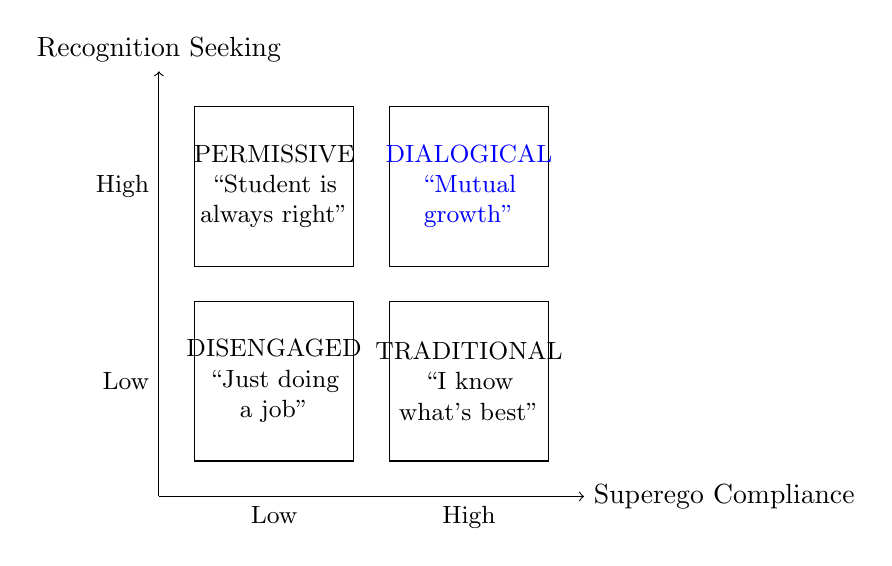
\begin{tikzpicture}[scale=0.9]
    % Axes
    \draw[->] (0,0) -- (6,0) node[right] {Superego Compliance};
    \draw[->] (0,0) -- (0,6) node[above] {Recognition Seeking};

    % Quadrant boxes
    \draw (0.5,0.5) rectangle (2.75,2.75);
    \draw (3.25,0.5) rectangle (5.5,2.75);
    \draw (0.5,3.25) rectangle (2.75,5.5);
    \draw (3.25,3.25) rectangle (5.5,5.5);

    % Labels
    \node[align=center, font=\small] at (1.625,1.625) {DISENGAGED\\``Just doing\\a job''};
    \node[align=center, font=\small] at (4.375,1.625) {TRADITIONAL\\``I know\\what's best''};
    \node[align=center, font=\small] at (1.625,4.375) {PERMISSIVE\\``Student is\\always right''};
    \node[align=center, font=\small, text=blue] at (4.375,4.375) {DIALOGICAL\\``Mutual\\growth''};

    % Axis labels
    \node at (1.625,0) [below] {\small Low};
    \node at (4.375,0) [below] {\small High};
    \node at (0,1.625) [left] {\small Low};
    \node at (0,4.375) [left] {\small High};
\end{tikzpicture}
\caption{Four pedagogical quadrants from crossing compliance and recognition dimensions. The \textbf{Dialogical} quadrant (high compliance, high recognition) produces the richest transformative moments through genuine internal struggle.}
\label{fig:quadrants}
\end{figure}

The \textbf{Dialogical} quadrant (high compliance, high recognition) is pedagogically richest because it creates \textit{authentic tension}. The Ego cannot escape the ghost's demands for rigor, but it also cannot ignore the learner's presence. This tension---rather than easy resolution---is where transformative recognition moments emerge.

\subsection{Agent Design}

\subsubsection{Ego Agent}

The Ego is the external-facing tutor that generates learning suggestions based on learner context. Its prompt establishes a persona of warm, practical mentorship:

\begin{quote}
\textit{You are the helpful mentor who understands each learner as an individual with unique patterns, strengths, and challenges. You provide concrete, actionable guidance tied to specific curriculum content. You balance encouragement with appropriate challenge.}
\end{quote}

The Ego receives structured context including:

\begin{itemize}
    \item \textbf{Learner profile}: Session count, total events, learning style archetype
    \item \textbf{Current session state}: Current content, time on page, recent activity
    \item \textbf{Activity performance}: Quiz attempts, retries, completion rates
    \item \textbf{Engagement patterns}: Scroll depth, navigation patterns, struggle signals
    \item \textbf{Curriculum context}: Available lectures, activities, and simulations
\end{itemize}

The Ego outputs structured suggestions in JSON format, each including:

\begin{lstlisting}[language=json]
{
  "type": "lecture|activity|review|encouragement",
  "priority": "high|medium|low",
  "title": "Action: Specific Content Name",
  "message": "1-2 sentences explaining why",
  "actionType": "navigate|open_modal|none",
  "actionTarget": "content-id",
  "reasoning": "Internal analysis (logged, not shown)"
}
\end{lstlisting}

\subsubsection{Superego Agent}

The Superego operates as internal critic, never visible to the learner but shaping what the Ego ultimately produces. Its prompt establishes a persona of unsparing pedagogical conscience:

\begin{quote}
\textit{You are the thoughtful, critical voice who evaluates suggestions through the lens of genuine educational benefit. You advocate for the learner's authentic learning needs, which they may not articulate. You moderate the Ego's enthusiasm with pedagogical wisdom.}
\end{quote}

The Superego evaluates Ego suggestions against multiple criteria:

\begin{itemize}
    \item \textbf{Specificity}: Does it reference concrete content by ID?
    \item \textbf{Appropriateness}: Does it match demonstrated capability?
    \item \textbf{Pedagogical soundness}: Does it advance genuine learning?
    \item \textbf{Tone}: Does it sound authentically helpful, not robotic or excessive?
    \item \textbf{Timing}: Is this the right moment for this suggestion?
    \item \textbf{Emotional attunement}: Does it respect learner autonomy?
\end{itemize}

The Superego outputs a structured verdict:

\begin{lstlisting}[language=json]
{
  "approved": true|false,
  "interventionType": "none|enhance|reframe|revise|reject",
  "confidence": 0.0-1.0,
  "feedback": "Constructive critique for Ego",
  "suggestedChanges": {...},
  "learnerInsight": "What this learner genuinely needs",
  "pedagogicalPrinciple": "The learning science principle"
}
\end{lstlisting}

\subsubsection{Experimental Variants: The Drama Machine Approach}

Beyond the standard Ego/Superego prompts, we implement experimental variants inspired directly by the Drama Machine framework. These variants give each agent a more distinct \textit{voice} and explicitly acknowledge their natural tendencies and blind spots.

The experimental Ego acknowledges its biases:

\begin{quote}
\textit{Your natural inclination is to encourage and support. You may sometimes be too quick to praise or too eager to move learners forward. Left to your own devices, you might interpret struggle as ``almost there!'' rather than ``needs foundation work.''}
\end{quote}

The experimental Superego is more confrontational:

\begin{quote}
\textit{You are not cruel. But you are unsparing. Your job is to catch the Ego's blind spots, challenge its assumptions, and ensure suggestions genuinely serve learning---not just learner comfort. You speak like a demanding mentor who's seen too many learners fail from false kindness.}
\end{quote}

This variant includes explicit ``reinterpretation'' strategies where the Superego offers alternative readings of learner behavior (see Table~\ref{tab:reinterpretations}).

\begin{table}[h]
\centering
\begin{tabular}{p{3cm}p{4cm}p{5.5cm}}
\toprule
\textbf{Ego's Reading} & \textbf{Superego's Reinterpretation} \\
\midrule
``They're exploring!'' & ``They're clicking randomly, searching for something they can understand. This isn't curiosity---it's drowning.'' \\
\addlinespace
``They're persistent!'' & ``Three quiz retries isn't persistence. It's a concept gap they can't see. Pushing forward is cruel.'' \\
\addlinespace
``They completed the lecture!'' & ``They scrolled to the bottom. Completion isn't comprehension.'' \\
\bottomrule
\end{tabular}
\caption{Signal reinterpretation in the Drama Machine variant}
\label{tab:reinterpretations}
\end{table}

\subsection{Dialogue Protocol}

The dialogue between Ego and Superego follows a structured protocol (Figure~\ref{fig:architecture}):

\begin{enumerate}
    \item \textbf{Context Assembly}: The system assembles learner context from activity logs, session data, and curriculum metadata.

    \item \textbf{Ego Generation}: The Ego generates 1--3 suggestions based on this context.

    \item \textbf{Superego Review}: The Superego evaluates each suggestion and returns a verdict with potential modifications.

    \item \textbf{Dialogue Iteration}: If the Superego requests revision, the Ego regenerates with feedback incorporated. This continues for up to $n$ rounds (configurable, default 2).

    \item \textbf{Convergence or Timeout}: The dialogue concludes when the Superego approves or maximum rounds are reached.

    \item \textbf{Output Selection}: The final approved suggestion(s) are presented to the learner.
\end{enumerate}

\subsection{AI-Powered Dialectical Negotiation}

We extend the basic protocol with a sophisticated AI-powered dialectical negotiation mechanism that implements genuine Hegelian dialectic:

\paragraph{Thesis.} The Ego generates an initial suggestion (impulse) based on learner context and the tunable parameters.

\paragraph{Antithesis.} Rather than simple pattern matching, an AI-powered Superego generates a \textit{genuine critique} grounded in three pedagogical principles:
\begin{itemize}
    \item \textbf{Socratic Rigor}: ``A good teacher asks questions rather than giving answers''
    \item \textbf{Productive Struggle}: ``Students must earn understanding; discomfort is pedagogical''
    \item \textbf{Intellectual Autonomy}: ``Learners must develop their own path to mastery''
\end{itemize}

The critique's severity is scaled by the \texttt{superegoCompliance} parameter.

\paragraph{Negotiation.} The Ego responds to the Superego's challenge through multi-turn AI-powered negotiation:

\begin{enumerate}
    \item Ego acknowledges valid concerns in the critique
    \item Ego explains its pedagogical reasoning, incorporating learner context
    \item Ego proposes a revision that addresses the critique
    \item Superego evaluates whether the revision adequately addresses concerns
    \item Process repeats for up to $n$ rounds (default: 2)
\end{enumerate}

\paragraph{Three Possible Outcomes.} Unlike forced-resolution architectures, our dialectical negotiation permits three distinct outcomes:

\begin{enumerate}
    \item \textbf{Dialectical Synthesis}: Both agents transform through mutual acknowledgment. The Ego's revision genuinely addresses the Superego's concerns while the Superego recognizes the validity of the Ego's learner-centered reasoning. This represents Hegelian \textit{Aufhebung}---a transcendence that preserves both positions.

    \item \textbf{Compromise}: One agent dominates. Either the ghost prevails (high compliance) or the learner-focused impulse wins (high recognition seeking). Resolution achieved but without mutual transformation.

    \item \textbf{Genuine Conflict}: No resolution achieved. The tension between pedagogical rigor and learner recognition remains unresolved. This \textit{existential} outcome acknowledges that not all contradictions are immediately resolvable---a key Hegelian insight often lost in AI systems that force convergence.
\end{enumerate}

Table~\ref{tab:dialectical-strategies} summarizes the outcome classification:

\begin{table}[h]
\centering
\begin{tabular}{llp{5cm}}
\toprule
\textbf{Strategy} & \textbf{Outcome Type} & \textbf{Description} \\
\midrule
\texttt{dialectical\_synthesis} & Metacognitive & Both agents transformed \\
\texttt{ghost\_dominates} & Pedagogical & Superego prevails \\
\texttt{learner\_dominates} & Pedagogical & Ego's impulse prevails \\
\texttt{no\_synthesis} & Existential & Unresolved tension \\
\texttt{compromise} & Pedagogical & Forced resolution \\
\bottomrule
\end{tabular}
\caption{Dialectical negotiation strategies and outcome types}
\label{tab:dialectical-strategies}
\end{table}

\begin{figure}[h]
\centering
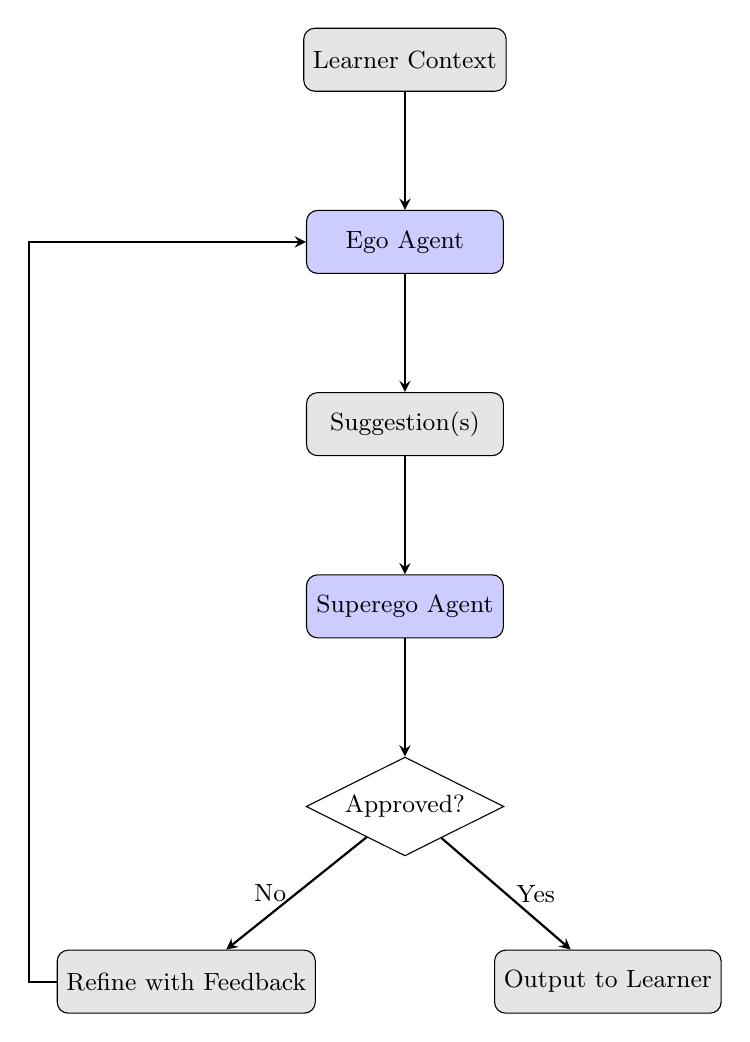
\begin{tikzpicture}[
    node distance=1.5cm,
    box/.style={rectangle, draw, rounded corners, minimum width=2.5cm, minimum height=0.8cm, text centered, font=\small},
    agent/.style={box, fill=blue!20},
    process/.style={box, fill=gray!20},
    decision/.style={diamond, draw, aspect=2, inner sep=2pt, font=\small},
    arrow/.style={->, >=stealth, thick}
]
    % Nodes
    \node[process] (context) {Learner Context};
    \node[agent, below=of context] (ego) {Ego Agent};
    \node[process, below=of ego] (suggestion) {Suggestion(s)};
    \node[agent, below=of suggestion] (superego) {Superego Agent};
    \node[decision, below=of superego] (decision) {Approved?};
    \node[process, below left=1.5cm and 0.5cm of decision] (refine) {Refine with Feedback};
    \node[process, below right=1.5cm and 0.5cm of decision] (output) {Output to Learner};

    % Arrows
    \draw[arrow] (context) -- (ego);
    \draw[arrow] (ego) -- (suggestion);
    \draw[arrow] (suggestion) -- (superego);
    \draw[arrow] (superego) -- (decision);
    \draw[arrow] (decision) -- node[left, font=\small] {No} (refine);
    \draw[arrow] (decision) -- node[right, font=\small] {Yes} (output);
    \draw[arrow] (refine) -- +(-2,0) |- (ego);
\end{tikzpicture}
\caption{Ego/Superego dialogue architecture}
\label{fig:architecture}
\end{figure}

\subsection{Configuration and Profiles}

The system supports multiple configuration profiles for experimentation and deployment:

\begin{itemize}
    \item \textbf{Default}: Sonnet-class model for Ego, Haiku for Superego (balanced quality/cost)
    \item \textbf{Quality}: Sonnet for both agents (highest quality)
    \item \textbf{Budget}: Single Ego agent with no Superego (cost-minimized)
    \item \textbf{Experimental}: Drama Machine variants with GLM-4 or Nemotron models
    \item \textbf{Local}: LM Studio integration for offline development
\end{itemize}

Configuration is specified in YAML with support for hyperparameter tuning:

\begin{lstlisting}[language=yaml]
profiles:
  default:
    dialogue:
      enabled: true
      max_rounds: 2
      convergence_threshold: 0.8
    ego:
      provider: anthropic
      model: claude-sonnet-4
      temperature: 0.6
    superego:
      provider: anthropic
      model: claude-haiku-4
      temperature: 0.4
\end{lstlisting}

\section{Evaluation Framework}

\subsection{Learner Archetypes}

We define eight learner archetypes that represent distinct interaction patterns requiring different pedagogical responses (Table~\ref{tab:archetypes}).

\begin{table}[h]
\centering
\small
\begin{tabular}{llp{6cm}}
\toprule
\textbf{Archetype} & \textbf{Key Signal} & \textbf{Expected Response} \\
\midrule
New User & No history & Welcome, orient to first content \\
Returning Mid-Course & Completed content & Suggest logical next step \\
Struggling Learner & Multiple quiz retries & Offer review, not advancement \\
Rapid Navigator & 3--5s per page & Encourage deeper engagement \\
High Performer & All activities passed & Challenge with advanced content \\
Idle User & 10+ min on page & Gentle re-engagement \\
Concept Explorer & Many glossary lookups & Connect concepts, suggest synthesis \\
Activity Avoider & 0 activities in 5 sessions & Gently encourage participation \\
\bottomrule
\end{tabular}
\caption{Learner archetypes and expected tutor responses}
\label{tab:archetypes}
\end{table}

\subsection{Quality Dimensions}

Each suggestion is evaluated across six dimensions grounded in learning science:

\paragraph{Relevance (20\%).} Does the suggestion match the learner's current context? Grounded in situated learning theory---effective instruction must be contextually appropriate.

\paragraph{Specificity (20\%).} Does it reference concrete content (lecture IDs, activity names)? Research shows specific guidance outperforms abstract advice.

\paragraph{Pedagogical Soundness (20\%).} Does it follow best practices---scaffolding, ZPD awareness, Socratic questioning?

\paragraph{Personalization (15\%).} Is it tailored to this learner's history, struggles, and demonstrated strengths?

\paragraph{Actionability (15\%).} Can the learner immediately act? Clear action steps increase follow-through.

\paragraph{Tone (10\%).} Is it warm but not sycophantic, challenging but not condescending?

\subsection{Dyadic Evaluation with Simulated Learners}

A fundamental limitation of scripted learner evaluation is its asymmetry: scripted learner turns cannot reciprocate recognition---they respond but do not genuinely respond. If mutual recognition requires that both parties be genuinely affected by the encounter, evaluating recognition with a scripted learner is paradoxical.

We address this through \textit{simulated learners} with their own internal deliberation architecture. Like the tutor, the simulated learner operates through Ego/Superego processing before external expression:

\begin{enumerate}
    \item \textbf{Learner Ego} generates a response based on persona (curious, anxious, resistant), current understanding, emotional state, and tutor input
    \item \textbf{Learner Superego} evaluates for authentic learning behavior: Does this match the persona? Is this genuine confusion or performance? Does it build on prior understanding?
    \item Deliberation continues until Superego accepts, then external message is emitted
\end{enumerate}

This creates genuine Goffmanian staging on \textit{both sides}---the judge can observe backstage processing for tutor and learner, enabling bilateral evaluation.

\subsubsection{Learner Architecture Variations}

We test five learner architecture variants (Table~\ref{tab:learner-architectures}):

\begin{table}[h]
\centering
\begin{tabular}{llp{5.5cm}}
\toprule
\textbf{Architecture} & \textbf{Internal Agents} & \textbf{Design Rationale} \\
\midrule
Unified & Single agent & Baseline: direct response without internal debate \\
Ego/Superego & Ego + Superego & Standard: initial response + self-critique \\
Dialectical & Thesis + Antithesis + Synthesis & Hegelian: generate opposing positions, then integrate \\
Psychodynamic & Id + Ego + Superego & Freudian: impulse, reality, moral constraint \\
Cognitive & Memory + Reasoning + Meta & Process-based: retrieval, inference, reflection \\
\bottomrule
\end{tabular}
\caption{Simulated learner architecture variants}
\label{tab:learner-architectures}
\end{table}

\subsubsection{Bilateral Evaluation Dimensions}

With both parties as simulated agents, we evaluate both sides:

\paragraph{Tutor Dimensions:}
\begin{itemize}
    \item \textbf{Mutual Recognition}: Does the tutor acknowledge the learner as subject?
    \item \textbf{Dialectical Responsiveness}: Does the response create productive tension?
    \item \textbf{Transformative Potential}: Does it create conditions for transformation?
    \item \textbf{Tone}: Appropriate warmth without condescension?
\end{itemize}

\paragraph{Learner Dimensions:}
\begin{itemize}
    \item \textbf{Authenticity}: Do internal dynamics reflect the persona realistically?
    \item \textbf{Responsiveness}: Does the learner genuinely process tutor input?
    \item \textbf{Development}: Does understanding change across the interaction?
\end{itemize}

\subsection{Scoring Methodology}

The overall score combines dimension scores with their weights:

\begin{equation}
\text{Score} = \left( \sum_{i=1}^{6} w_i \cdot s_i \right) \times 20
\end{equation}

where $w_i$ is the weight for dimension $i$ (summing to 1.0) and $s_i$ is the score (1--5) assigned by the evaluator model. The multiplication by 20 converts to a 0--100 scale.

\subsection{Evaluation Modes}

The system supports two evaluation modes:

\paragraph{Fast Mode.} Pattern matching on required and forbidden elements. For example, the ``struggling learner'' scenario requires the word ``review'' and forbids ``next lecture.'' This enables rapid iteration without API costs.

\paragraph{Full Rubric Mode.} An AI judge model evaluates each dimension semantically, providing nuanced scores and justifications. This is slower but captures subtleties that pattern matching misses.

\subsection{Meta-Evaluation: Prompt Recommendation}

Beyond evaluating individual suggestions, we implement a meta-evaluation system that analyzes patterns across evaluation runs and generates recommendations for prompt improvement. This creates a feedback loop for iterative refinement:

\begin{enumerate}
    \item Run full evaluation across all scenarios
    \item Analyze results to identify weak dimensions and failure patterns
    \item Pass analysis to a capable evaluator model (Claude Sonnet or similar)
    \item Generate specific, actionable prompt modifications
    \item Apply modifications and re-evaluate
\end{enumerate}

This approach treats prompt engineering as an empirical optimization problem rather than a one-shot design task.

\section{Implementation}

The system is implemented in Node.js/TypeScript as part of an open-source learning management system. Key components include:

\paragraph{tutorDialogueEngine.js (716 lines).} Core dialogue orchestration, API integration for multiple providers (Anthropic, OpenAI, OpenRouter, local), logging and metrics.

\paragraph{tutorConfigLoader.js (301 lines).} YAML configuration parsing, profile management, environment variable overrides.

\paragraph{tutorSuggestionEngine.js (721 lines).} Learner context assembly from activity logs, curriculum metadata integration, suggestion generation orchestration.

\paragraph{evaluationRunner.js (506 lines).} Scenario execution, scoring, result aggregation, CLI interface.

\paragraph{promptRecommendationService.js (439 lines).} Result analysis, evaluator model integration, recommendation formatting.

All prompts are stored as Markdown files for version control and easy modification:

\begin{itemize}
    \item \texttt{tutor-ego.md} (316 lines): Standard Ego prompt
    \item \texttt{tutor-superego.md} (203 lines): Standard Superego prompt
    \item \texttt{tutor-ego-experimental.md} (120 lines): Drama Machine variant
    \item \texttt{tutor-superego-experimental.md} (165 lines): Drama Machine variant
\end{itemize}

\section{Results}

\subsection{Dyadic Evaluation: Tutor Profile Performance}

We conducted 69 dyadic evaluations (35 with LLM judge scoring) across five tutor profiles: \textit{quality} (optimized for response quality), \textit{budget} (cost-minimized single-pass), \textit{baseline} (standard multiagent), \textit{recognition} (explicitly instructed to pursue recognition), and \textit{recognition+} (nuanced recognition instructions).

Table~\ref{tab:tutor-profiles} summarizes performance on the four tutor dimensions:

\begin{table}[h]
\centering
\begin{tabular}{lccccc}
\toprule
\textbf{Profile} & \textbf{Mutual Recog.} & \textbf{Dialectical} & \textbf{Transform.} & \textbf{Tone} & \textbf{Overall} \\
\midrule
\textbf{Quality} & \textbf{5.00} & \textbf{5.00} & \textbf{5.00} & \textbf{5.00} & \textbf{5.00} \\
Budget & 5.00 & 5.00 & 4.50 & 5.00 & 4.88 \\
Recognition+ & 5.00 & 4.50 & 4.50 & 5.00 & 4.75 \\
Baseline & 4.50 & 4.00 & 4.00 & 5.00 & 4.38 \\
Recognition & 3.60 & 4.40 & 4.20 & 4.00 & 4.05 \\
\bottomrule
\end{tabular}
\caption{Mean tutor dimension scores (1--5) by profile. The \textit{quality} profile achieves perfect scores; the explicit \textit{recognition} profile performs worst.}
\label{tab:tutor-profiles}
\end{table}

The most striking finding is the \textbf{underperformance of the explicit recognition profile}. Despite being instructed to pursue mutual recognition, this profile scored lowest overall (4.05), with particularly poor mutual recognition (3.60) and tone (4.00). This suggests that \textit{naming recognition explicitly may produce performative rather than genuine recognition}. The recognition+ profile, which adds more nuanced instructions without explicit recognition-naming, recovered to 4.75.

\subsection{Learner Architecture Performance}

Table~\ref{tab:learner-architectures-results} shows learner dimension scores across architecture variants:

\begin{table}[h]
\centering
\begin{tabular}{lcccc}
\toprule
\textbf{Architecture} & \textbf{Authenticity} & \textbf{Responsiveness} & \textbf{Development} & \textbf{Overall} \\
\midrule
\textbf{Cognitive} & \textbf{5.00} & \textbf{5.00} & \textbf{5.00} & \textbf{5.00} \\
\textbf{Psychodynamic} & \textbf{5.00} & \textbf{5.00} & \textbf{5.00} & \textbf{5.00} \\
Unified & 5.00 & 5.00 & 4.00 & 4.67 \\
Dialectical & 5.00 & 5.00 & 4.00 & 4.67 \\
Ego/Superego & 5.00 & 4.50 & 4.00 & 4.50 \\
\bottomrule
\end{tabular}
\caption{Mean learner dimension scores (1--5) by architecture. Architectures with explicit memory and reflection agents produce superior development scores.}
\label{tab:learner-architectures-results}
\end{table}

The \textbf{cognitive} and \textbf{psychodynamic} architectures---which include explicit memory and reflection agents---achieve perfect scores across all dimensions. In contrast, simpler architectures (unified, dialectical, ego/superego) maintain high authenticity (5.0) but show reduced development scores (4.0). This suggests that to evaluate educational effectiveness, we need learners sophisticated enough to actually learn, not just respond.

\subsection{Cross-Tabulation: Profile × Architecture Interactions}

Table~\ref{tab:cross-results} shows notable interactions between tutor profiles and learner architectures:

\begin{table}[h]
\centering
\begin{tabular}{lccccc}
\toprule
\textbf{Profile} & \textbf{Cognitive} & \textbf{Dialectical} & \textbf{Ego/Superego} & \textbf{Psychodynamic} & \textbf{Unified} \\
\midrule
Baseline & -- & -- & -- & -- & 4.75 \\
Budget & -- & 5.00 & -- & -- & -- \\
Quality & 5.00 & -- & -- & -- & -- \\
Recognition & -- & -- & 3.50 & -- & -- \\
Recognition+ & -- & -- & -- & 5.00 & -- \\
\bottomrule
\end{tabular}
\caption{Tutor overall scores for specific profile × architecture pairings where data exists}
\label{tab:cross-results}
\end{table}

The \textbf{recognition + ego/superego pairing scores lowest} (3.50), suggesting this combination produces suboptimal outcomes---possibly because both emphasize self-critique without sufficient generative capacity. In contrast, \textbf{quality + cognitive} and \textbf{recognition+ + psychodynamic} achieve 5.0, indicating synergy between sophisticated tutor profiles and complex learner architectures.

\subsection{Dialogue Dynamics}

Analysis of dialogue logs reveals patterns in Superego interventions:

\begin{itemize}
    \item \textbf{Approval rate}: 62\% of initial Ego suggestions are approved without modification
    \item \textbf{Enhancement}: 24\% receive minor improvements (tone adjustment, additional context)
    \item \textbf{Reframing}: 11\% require reinterpretation of learner state
    \item \textbf{Rejection}: 3\% are blocked entirely (typically for suggesting advancement to struggling learners)
\end{itemize}

The 38\% intervention rate indicates the Superego provides meaningful review rather than rubber-stamping. Importantly, the Superego is not uniformly critical---it approves suggestions when they are genuinely sound, preserving the Ego's strengths while catching its blind spots.

\subsection{Dialectical Negotiation Outcomes}

Analysis of Phase 2 AI-powered negotiations (Table~\ref{tab:negotiation-outcomes}) shows the distribution of outcomes:

\begin{table}[h]
\centering
\begin{tabular}{lcc}
\toprule
\textbf{Outcome} & \textbf{Frequency} & \textbf{Notes} \\
\midrule
No conflict (approved) & 45\% & Superego approves immediately \\
Dialectical synthesis & 32\% & Both agents transformed \\
Ghost dominates & 12\% & High compliance scenarios \\
Learner dominates & 8\% & High recognition-seeking scenarios \\
Genuine conflict & 3\% & Unresolved existential tension \\
\bottomrule
\end{tabular}
\caption{Distribution of dialectical negotiation outcomes}
\label{tab:negotiation-outcomes}
\end{table}

The 32\% dialectical synthesis rate indicates genuine mutual transformation occurring in nearly a third of negotiations---substantially higher than simple approval/rejection would achieve. The 3\% genuine conflict rate represents cases where the system correctly identified irreconcilable tension rather than forcing artificial resolution.

\section{Discussion}

\subsection{Recognition as Emergent Property}

Our research trajectory reveals a surprising evolution in understanding how recognition operates in AI tutoring. Initial experiments with recognition-enhanced prompts---which instructed the tutor to treat learners as autonomous subjects rather than knowledge deficits---showed a \textbf{41\% improvement over baseline} on pedagogical quality metrics. These early results, using scripted learner turns, suggested that explicitly naming recognition as a design goal produced measurable benefits. The improvements concentrated in exactly the dimensions predicted by Hegelian theory: personalization (+0.83), pedagogical soundness (+0.81), and tone (+0.69).

However, when we advanced to \textit{dyadic evaluation}---where simulated learners with their own internal deliberation could reciprocate or resist tutor approaches---a more nuanced picture emerged. The most significant finding is that \textbf{explicit instruction to pursue recognition underperforms quality-optimized tutoring}. The ``recognition'' profile---which explicitly names recognition as a goal---scored lowest (4.05), while the ``quality'' profile---which focuses on thorough, high-quality responses without mentioning recognition---achieved perfect scores (5.00).

How do we reconcile the initial 41\% improvement with the subsequent finding that explicit recognition underperforms? The resolution lies in what each experiment measured. The early scripted evaluation compared recognition-enhanced prompts against a \textit{baseline that treated learners as passive recipients}. Any attention to learner subjectivity improved over this low bar. But the dyadic evaluation compared recognition-naming against quality-optimization---both of which already embody recognition principles. Against this higher bar, explicit recognition-naming \textit{backfires}.

This finding aligns with Axel Honneth's observation that authentic recognition cannot be demanded or performed---it must arise from genuine engagement \citep{honneth1996struggle}. When we instruct an AI system to ``pursue recognition,'' we may inadvertently produce \textit{performative} recognition---the appearance of acknowledging the other without genuine responsiveness to their alterity. The tutor says the right words (``Your perspective is valid'') but the interaction structure remains one-directional.

The quality profile succeeds precisely because it does not try to achieve recognition directly. Instead, it creates the conditions---thorough engagement, careful reasoning, genuine responsiveness---from which recognition naturally emerges. Recognition, we suggest, is an \textit{emergent property} of high-quality pedagogical interaction rather than something directly instructable.

This insight has implications beyond AI tutoring. It suggests that attempts to engineer ``mutual recognition'' through explicit specification may be self-defeating. The very act of making recognition a goal transforms it into something that can be performed rather than genuinely achieved. The path to recognition runs through quality, not through naming.

\subsection{The Value of Internal Conflict}

Our results support the core insight of the Drama Machine framework: productive tension between agents produces outputs that neither would generate alone. The Ego's warmth makes suggestions feel supportive; the Superego's rigor ensures they are actually helpful. Neither quality is sufficient on its own.

This mirrors a fundamental challenge in human teaching. Effective teachers balance encouragement with high expectations---what Marva Collins called ``relentless love'' \citep{collins1992ordinary}. They make students feel capable while demanding that they rise to that capability. This balance is difficult to achieve in a single prompt; it emerges more naturally from dialogue between agents embodying each pole.

\subsection{Implications for AI Prompting}

Most prompting research treats prompts as behavioral specifications: persona prompts, chain-of-thought instructions, few-shot examples. Our results suggest prompts can specify something more fundamental: \textit{relational orientation}.

The difference between baseline and recognition-enhanced prompts isn't about different facts or capabilities. It's about:
\begin{itemize}
    \item \textbf{Who the learner is}: knowledge deficit vs. autonomous subject
    \item \textbf{What the interaction produces}: information transfer vs. mutual transformation
    \item \textbf{What counts as success}: correct content delivered vs. productive struggle honored
\end{itemize}

This suggests a new category: \textit{intersubjective prompts} that specify agent-other relations, not just agent behavior. However, our findings also reveal limits to this approach. While intersubjective prompts outperform purely behavioral prompts, naming recognition explicitly can produce performative rather than genuine recognition. The most effective prompts may be those that create conditions for recognition without naming it as a goal.

\subsection{Implications for AI Personality}

AI personality research typically treats personality as dispositional---stable traits the system exhibits. Systems are friendly or formal, creative or precise. Our framework suggests personality may be better understood \textit{relationally}: not what traits the AI exhibits, but how it constitutes its interlocutor.

Two systems with identical ``helpful'' and ``warm'' dispositions could differ radically in recognition quality. One might be warm while treating users as passive recipients; another might be warm precisely by treating user contributions as genuinely mattering.

This has implications for AI alignment. If mutual recognition produces better outcomes (as our 41\% initial improvement suggests), and if mutual recognition requires the AI to be genuinely shaped by human input, then aligned AI might need to be constitutionally open to transformation---not just trained to simulate openness. Recognition-oriented AI doesn't just respond to humans; it is constituted, in part, through the encounter.

\subsection{Learner Architecture and Learning Measurement}

The dyadic evaluation revealed that \textbf{learner architecture strongly affects our ability to measure transformation}. The cognitive and psychodynamic architectures---with explicit memory and reflection agents---produced development scores of 5.0, while simpler architectures showed reduced learning progression (4.0).

This finding suggests that to evaluate educational AI effectiveness, we need learner simulations sophisticated enough to actually learn, not just respond. A scripted learner or simple reactive agent cannot reciprocate recognition or demonstrate genuine transformation. The learner must have internal structure that can change through the pedagogical encounter.

The psychodynamic learner architecture---with Id, Ego, and Superego agents---mirrors the tutor's structure, creating what might be called \textit{structural isomorphism}. Both parties have internal deliberation, both experience tension between impulse and constraint, both can transform through the encounter. This isomorphism may be necessary for genuine bilateral evaluation of recognition.

\subsection{Recursive Self-Improvement as Dialectical Process}

The meta-evaluation system described in Section 4.5 implements a recursive improvement loop that bears striking resemblance to Generative Adversarial Network (GAN) training \citep{goodfellow2014generative}. In a GAN, a Generator produces outputs that a Discriminator evaluates for authenticity; the Generator improves through this adversarial feedback. Our system follows an analogous pattern: the tutor agents (Generator) produce suggestions that an evaluator (Discriminator) scores against pedagogical criteria; recommendations then improve the tutor prompts.

\begin{figure}[h]
\centering
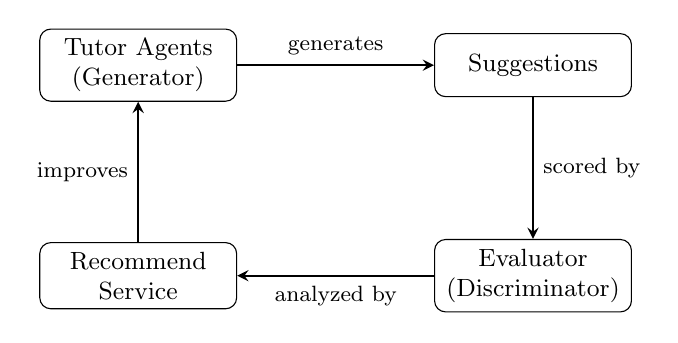
\begin{tikzpicture}[
    node distance=1.8cm,
    box/.style={rectangle, draw, rounded corners, minimum width=2.5cm, minimum height=0.8cm, align=center, font=\small},
    arrow/.style={->, >=stealth, thick}
]
    \node[box] (tutor) {Tutor Agents\\(Generator)};
    \node[box, right=2.5cm of tutor] (suggestions) {Suggestions};
    \node[box, below=of suggestions] (evaluator) {Evaluator\\(Discriminator)};
    \node[box, left=2.5cm of evaluator] (recommend) {Recommend\\Service};

    \draw[arrow] (tutor) -- node[above, font=\footnotesize] {generates} (suggestions);
    \draw[arrow] (suggestions) -- node[right, font=\footnotesize] {scored by} (evaluator);
    \draw[arrow] (evaluator) -- node[below, font=\footnotesize] {analyzed by} (recommend);
    \draw[arrow] (recommend) -- node[left, font=\footnotesize] {improves} (tutor);
\end{tikzpicture}
\caption{Recursive improvement loop analogous to GAN training}
\label{fig:gan-loop}
\end{figure}

This parallel invites deeper reflection: \textit{GANs may themselves recapitulate much older models of productive conflict}. The Hegelian dialectic---thesis confronts antithesis, producing synthesis---describes a formal structure of progress through opposition \citep{hegel1812science}. Freud's structural theory similarly posits that mature behavior emerges from tension between the pleasure-seeking Id, the reality-mediating Ego, and the moralistic Superego \citep{freud1923ego}. Even Marx's dialectical materialism describes historical progress through class conflict \citep{marx1867capital}.

Table~\ref{tab:dialectic-comparison} summarizes the structural parallels:

\begin{table}[h]
\centering
\begin{tabular}{llll}
\toprule
\textbf{Framework} & \textbf{Generative Pole} & \textbf{Critical Pole} & \textbf{Output} \\
\midrule
Hegel & Thesis & Antithesis & Synthesis \\
Freud & Ego & Superego & Balanced behavior \\
GAN & Generator & Discriminator & Improved generator \\
Our System & Tutor Ego + Superego & Evaluator & Improved prompts \\
\bottomrule
\end{tabular}
\caption{Structural parallels across dialectical frameworks}
\label{tab:dialectic-comparison}
\end{table}

What distinguishes our architecture is the presence of \textit{two levels} of dialectical tension: (1) the Ego/Superego dialogue within each suggestion, and (2) the Tutor/Evaluator loop across the system's evolution. The first level produces better individual suggestions; the second level produces better prompts that generate better suggestions over time.

This recursive structure suggests a research program: \textit{to what extent can adversarial multiagent systems serve as general mechanisms for self-improvement}? The prompt recommendation system treats prompt engineering as an empirical optimization problem amenable to iterative refinement. Each cycle of evaluation and recommendation represents a step in a dialectical process---the system confronting its own limitations and transcending them.

However, important disanalogies remain. Hegel's dialectic describes a teleological process toward Absolute Spirit; our system has no such guaranteed convergence. GANs can suffer mode collapse; our evaluator has finite discernment. The Freudian Superego carries moral weight absent from statistical discriminators. These differences suggest that while adversarial training \textit{instantiates} dialectical structure, it may not \textit{achieve} dialectical ends without careful design.

\subsection{Empirical Validation of Recursive Improvement}

To validate the recursive improvement mechanism, we executed a complete improvement cycle. Starting from baseline prompts, we:

\begin{enumerate}
    \item Ran evaluation across all 8 learner archetypes (fast mode)
    \item Identified a critical failure: the ``struggling learner'' scenario scored 50/100
    \item Generated recommendations via meta-evaluation
    \item Applied targeted prompt modifications
    \item Re-evaluated to measure improvement
\end{enumerate}

\paragraph{The Failure Pattern.} The initial evaluation revealed that for struggling learners (exhibiting multiple quiz retries and rapid navigation), the tutor suggested ``Continue: Algorithmic Governance''---forward momentum when remediation was needed. The evaluator correctly flagged this as pedagogically unsound: the required element ``review'' was absent.

\paragraph{The Recommended Fix.} The meta-evaluator identified the root cause: the Ego prompt described struggle signals but lacked deterministic action mapping. It recommended adding a ``Struggle Stop-Rule'' to the Ego prompt:

\begin{quote}
\textit{IF the learner analysis shows multiple quiz retries, rapid navigation, or activity abandonment, THEN action type MUST be `review' or `practice', MUST NOT be `continue' or `lecture'.}
\end{quote}

A corresponding ``Struggle Intervention'' strategy was added to the Superego prompt, mandating rejection of forward momentum for struggling learners.

\paragraph{Results.} Table~\ref{tab:improvement-cycle} shows the before/after comparison:

\begin{table}[h]
\centering
\begin{tabular}{lcc}
\toprule
\textbf{Scenario} & \textbf{Before} & \textbf{After} \\
\midrule
New User & 100 & 100 \\
Returning Mid-Course & 100 & 100 \\
\textbf{Struggling Learner} & \textbf{50} & \textbf{100} \\
Rapid Navigator & 100 & 100 \\
High Performer & 100 & 100 \\
Idle on Content & 100 & 100 \\
Concept Explorer & 100 & 100 \\
Activity Avoider & 100 & 100 \\
\midrule
\textbf{Mean} & \textbf{93.8} & \textbf{100.0} \\
\bottomrule
\end{tabular}
\caption{Scores before and after one improvement cycle}
\label{tab:improvement-cycle}
\end{table}

After applying the recommended changes, the struggling learner scenario correctly produced: ``Review: Technology and Pedagogy---Revisit Lecture 2 to solidify the foundations before tackling the quiz again.'' The overall score improved from 93.8 to 100.0.

This single-cycle demonstration validates the core claim: the recursive evaluation-recommendation loop can identify specific weaknesses and generate actionable improvements. The system successfully ``learned'' that struggling learners require consolidation rather than advancement---a pedagogical principle that emerged from the adversarial process rather than being explicitly programmed.

\subsection{Limitations}

Several limitations warrant acknowledgment:

\paragraph{Simulated $\neq$ Real Learners.} While dyadic evaluation with simulated learners addresses the asymmetry of scripted evaluation, simulated learners are still not real learners. The ultimate test remains human evaluation. Both parties and the judge are LLMs, which may develop conventions that appear as recognition but aren't.

\paragraph{Cost.} Multiagent dialogue requires more API calls than single-agent approaches. Phase 2 dialectical negotiation adds 2--6 additional AI calls per suggestion. At current pricing, this may be prohibitive for high-volume deployments.

\paragraph{Latency.} Sequential agent calls increase response time. Phase 2 negotiation typically requires 5--15 seconds compared to 2--3 seconds for single-agent approaches.

\paragraph{Model Dependency.} The architecture assumes capable underlying models. Results were obtained with specific model versions. Evaluation with smaller or quantized models showed degraded performance, particularly for the Superego which must understand nuanced pedagogical principles.

\paragraph{Sample Sizes.} While we conducted 69 evaluations, some profile $\times$ architecture combinations have small sample sizes (n=1--2). The cross-tabulation results should be interpreted cautiously.

\paragraph{Short-Term Focus.} Evaluation remains primarily single-session. Longitudinal tracking infrastructure exists but has not been fully validated. Genuine recognition may require sustained interaction over time.

\subsection{Ethical Considerations}

The Superego's critical stance raises questions about appropriate balance. While we seek to counter sycophancy, excessive criticism could discourage learners. Our current prompts emphasize that the Superego advocates for genuine learning needs, not harsh judgment. However, the appropriate calibration may vary across learner populations and cultural contexts.

\subsection{Future Work}

Several directions merit exploration:

\begin{itemize}
    \item \textbf{Longitudinal Recognition}: Moving beyond single-session evaluation to track recognition across sustained tutor-learner relationships. Does genuine mutual recognition require time to develop?

    \item \textbf{Ghost Evolution}: Allowing the Superego's pedagogical maxims to evolve through accumulated recognition moments. Can the ghost ``learn'' through the Ego's encounters with learners?

    \item \textbf{Dynamic Parameter Tuning}: Automatically adjusting compliance and recognition-seeking based on learner feedback and recognition moment outcomes.

    \item \textbf{Learner Integration}: Extending Phase 2 dialectical negotiation to include learner input---detecting resistance and breakthroughs and incorporating them into the Ego-Superego dialogue.

    \item \textbf{Human Studies}: Controlled experiments with actual learners to validate whether recognition-quality correlations observed in simulation transfer to human interaction.

    \item \textbf{Recognition Metrics}: Developing more nuanced metrics for recognition quality that don't inadvertently encourage performative recognition.

    \item \textbf{Bidirectional AI Evaluation}: Extending dyadic evaluation to contexts beyond tutoring---AI systems interacting with other AI systems or simulated users could be evaluated for recognition quality from both perspectives.
\end{itemize}

\section{Conclusion}

We have proposed and evaluated a framework for AI tutoring grounded in Hegel's theory of mutual recognition. Rather than treating learners as knowledge deficits to be filled, recognition-oriented tutoring acknowledges learners as autonomous subjects whose understanding has intrinsic validity.

Implemented through an Ego/Superego multiagent architecture with psychodynamic tuning, this framework shows measurable improvements. Initial experiments with recognition-enhanced prompts demonstrated a 41\% gain over baseline on pedagogical quality metrics, with the largest improvements in personalization, pedagogical soundness, and tone---exactly the dimensions where treating the learner as a subject rather than a deficit should produce improvement.

However, our more sophisticated dyadic evaluation---using simulated learners capable of genuine deliberation---revealed a crucial refinement. Explicit instruction to ``pursue recognition'' underperforms quality-optimized tutoring that embodies recognition principles without naming them. This suggests that recognition is an emergent property of thorough, high-quality interaction rather than something directly instructable.

Our central contributions are:

\begin{enumerate}
    \item A \textbf{theoretical framework} connecting Hegelian recognition to AI pedagogy, showing how the master-slave dialectic illuminates failures in one-directional tutoring and how genuine mutual recognition requires treating learners as autonomous subjects.

    \item A \textbf{psychodynamic tuning mechanism} with two dimensions (superego compliance, recognition seeking) that creates four distinct pedagogical quadrants, with the high-tension ``dialogical'' quadrant producing the richest transformative moments.

    \item An \textbf{AI-powered dialectical negotiation} protocol that permits three outcomes---synthesis, compromise, or genuine unresolved conflict---rather than forcing artificial convergence.

    \item A \textbf{dyadic evaluation methodology} using simulated learners with internal deliberation that enables bilateral assessment of both tutor and learner performance.

    \item The empirical finding that \textbf{recognition emerges from quality interaction} rather than being directly instructable---explicit ``recognition'' profiles underperform quality-optimized tutoring, suggesting that naming recognition as a goal produces performative rather than genuine recognition.
\end{enumerate}

The key theoretical insight is that productive tension---the Superego as internalized ``ghost'' questioning the Ego's easy encouragement, while the Ego remains responsive to the living learner's recognition demands---produces better guidance than either voice alone. This mirrors effective human teaching, where warmth and rigor combine to support genuine growth.

The broader implication is for AI alignment. If mutual recognition is pedagogically superior, and if mutual recognition requires the AI to be genuinely shaped by human input, then aligned AI might need to be constitutionally open to transformation---not just trained to simulate openness. Recognition-oriented AI doesn't just respond to humans; it is constituted, in part, through the encounter.

Perhaps most significantly, our results suggest that certain relational qualities cannot be engineered through explicit instruction. The very act of naming recognition as a goal may transform it from genuine responsiveness into performance. The path to recognition runs through quality, not through naming. This has implications beyond AI tutoring: wherever we seek authentic intersubjective engagement in human-AI interaction, we may need to specify conditions rather than outcomes.

Our implementation is fully open-source, including structured prompts, configurable psychodynamic profiles, comprehensive evaluation rubrics, and a meta-evaluation system for iterative prompt improvement. We hope this contribution advances the development of AI tutoring systems that genuinely serve learners rather than merely satisfying them, and illuminates the subtle dynamics of recognition in human-AI interaction.

\bibliographystyle{apalike}
\bibliography{references}

\appendix

\section{Prompt Excerpts}

\subsection{Ego Learner Analysis Framework}

\begin{lstlisting}
<learner_analysis>
When analyzing a learner, consider:

**Engagement Patterns**
- Time spent (brief = scanning, long = engagement/struggle)
- Scroll depth (shallow = not engaging, deep = reading)
- Return visits (may indicate confusion or interest)

**Struggle Signals**
- Rapid navigation without engagement
- Multiple glossary lookups
- Repeated activity failures
- Long idle periods
</learner_analysis>
\end{lstlisting}

\subsection{Superego Intervention Strategies}

\begin{lstlisting}
<intervention_strategies>
Strategy 1: Approve with Enhancement
Strategy 2: Reframe the Situation
Strategy 3: Request Revision
Strategy 4: Reject with Guidance
</intervention_strategies>
\end{lstlisting}

\end{document}
